\section{Análisis y Conclusiones}
\label{sec:analisis}

\subsection*{Aclaración sobre las mediciones}
Hay que aclarar que ninguna de las dos mediciones, \textit{tiempo.h} ni \textit{callgrind}, son un reflejo al 100\% de la diferencia de rendimiento entre ambas versiones de un mismo efecto. Por un lado, \textit{tiempo.h} está sujeto a las vicisitudes del scheduling del OS en que se corra; si bien se trató de minimizar este efecto cerrando todos los programas en la computadora donde se estaban realizando las mediciones, además de corriendo los algoritmos una gran cantidad de veces (100 iteraciones), sigue sin ser una medición perfecta. 
Por otro lado, el costo total de instrucciones con \textit{callgrind} incluye también los llamados a la API libsndfile, donde en algunos casos (viendo los archivos en \textit{callgrind/}) se puede ver que son gran parte del aporte total, por lo que el rendimiento no es realmente ``4 veces mejor'' en \textbf{Assembler} que en \textbf{C}. Ejemplificaremos esto con las figuras \ref{fig:delay-overhead-libsndfile} y \ref{fig:delay-overhead-libsndfile-asm}.

\begin{figure}[H]
    \centering
    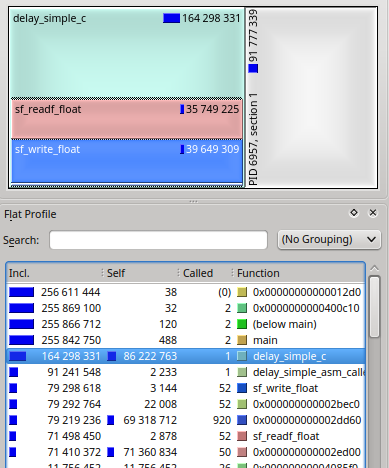
\includegraphics[scale=0.7]{imagenes/delay-overhead-libsndfile.png}
    \label{fig:delay-overhead-libsndfile}
    \caption{Delay libsndfile Overhead C}
\end{figure}

En la figura \ref{fig:delay-overhead-libsndfile}, la columna de la izquierda, con 3 filas, describe lo que pasa en el llamado a la función \textit{delay\_simple\_c}. Su costo total (164.000.000), está compuesto en un poco menos del 50\% ($35.000.000+40.000.000 = 75.000.000$) por los llamados a lectura y escritura de archivos.

\begin{figure}[H]
    \centering
    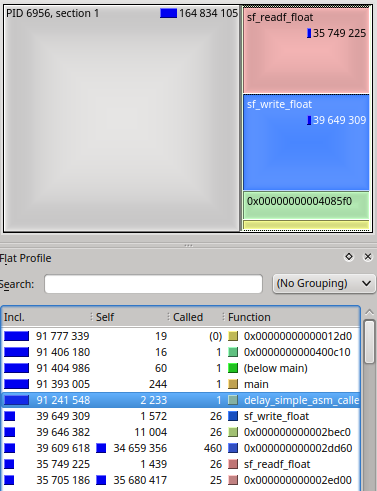
\includegraphics[scale=0.7]{imagenes/delay-overhead-libsndfile-asm.png}
    \label{fig:delay-overhead-libsndfile-asm}
    \caption{Delay libsndfile Overhead ASM}
\end{figure}

En la figura \ref{fig:delay-overhead-libsndfile-asm}, la columna de la derecha describe la función \textit{delay\_simple\_asm\_caller}; en este caso, la fila verde representa el código en el archivo \textbf{delay.asm}, y es notorio que su costo es muchísimo menor que los llamados a las funciones de la librería \textbf{libsndfile}, que son los que engrosan la cantidad total de instrucciones. 

\subsection{Análisis}
En casi todos los gráficos presentados en la sección Resultados \ref{sec:resultados}) se puede observar que la diferencia de rendimiento de haber aplicado los efectos en \textbf{ASM} frente a \textbf{C} es notoria, siendo más rápido Assembler, obteniéndose entonces el resultado esperado. La proporción de la variación varía según se vean los resultados de la librería \textbf{tiempo.h}, o los de \textbf{callgrind}. Dado que se está trabajando de a 4 muestras a la vez, se esperaría un rendimiento como mucho hasta 4 veces mejor. La librería \textbf{tiempo.h} excede esta mejoría, por motivos que desconozco, mientras que el uso de \textbf{callgrind} representa casi siempre una mejoría de entre 2.5 a 3 veces, más acorde al rendimiento esperado; sin embargo, hay que tener en cuenta que hay una cantidad fija de instrucciones que se encuentran en C y ASM, debido a la utilización de libsndfile, además de, potencialmente, otras.

El único resultado (y la razón por la que se puso \textit{casi} al inicio del párrafo anterior) que llama la atención es el de la \fullref{fig:resultados-flanger-tiempo}, donde \textbf{ASM} se muestra considerablemente peor que \textbf{C}; sin embargo, en la medición \fullref{fig:resultados-flanger-callgrind}, más confiable, se muestra que efectivamente es menos ``costosa'' la implementación en \textbf{ASM}.

Cabe destacar que en varios de los efectos (Vibrato, WahWah por ejemplo) se requiere en un ciclo N acceder a muestras no contiguas del ciclo N-1, lo que imposibilita en gran medida una paralelización completa, ya que el acceso a esos índices específicos se hace por separado, aumentando considerablemente la cantidad de accesos a memoria, lo que ocasiona cierta pérdida de rendimiento (aunque por suerte, no lo suficiente como para haber ocasionado problemas, por lo que se vio en los resultados).

\subsection{Conclusiones}
El TP probó ser bastante largo, por el proceso de desarrollo en sí, explicado en \fullref{subsec:intro-desarrollo}. El proceso iterativo de encontrar un algoritmo inteligible que provocara un efecto convincente y adecuado (que no es fácil, dado que muchas soluciones son privadas), aplicar el primer acercamiento en R/M/S, bajarlo de nivel a C y hacer que funcione leyendo un archivo de a partes (lo que llevó a pensar algunas soluciones específicas, como el caso del buffer circular en Vibrato), para finalmente ver cómo paralelizarlo en Assembler, es bastante largo.

A la vez, hubo muchas versiones de cada uno de los efectos, basadas en las mejoras que se iban haciendo en unos y que hacían dar cuenta que era posible mejorar los previamente hechos. Por ejemplo, en un principio en el código en \textbf{assembler} había dos ciclos completamente distintos para manejar archivos de entrada \textbf{stereo} y \textbf{mono} por el otro lado (recordemos que en el primer caso, es necesario ``convertirlo a mono'' para poder tener un canal libre en la salida y guardar la señal húmeda allí). Durante el desarrollo de un efecto posterior, se pensó en una solución más fácil: sólo separar el manejo de llevar la entrada desde memoria a un registro, y a partir de ahí las operaciones iban a ser como si se estuviera trabajando sobre una señal mono. Esta mejora se hizo retroactiva a los primeros efectos diseñados, lo que agregó bastante tiempo al desarrollo, pero redujo y simplificó el código de manera notables. Otra mejora fue la estandarización de los nombres de los registros en los distintos efectos.

Por otro lado, programar en \textbf{assembler} no es para nada fácil. Hubo bastantes problemas con casos bordes (cuando no se podían procesar 4 frames en simultáneo, por ejemplo), cosas que pasaban en archivos \textbf{stereo} y no en \textbf{mono} (sobre todo cuando los ciclos estaban separados), y el debugging para saber cómo se estaban realizando las operaciones y si coincidían los resultados de cada muestra de la señal entre \textbf{ASM} y \textbf{C} se hizo bastante engorroso (por lo insatisfactorio que resultaba el debugging con \textbf{ddd} (explicado en \ref{subsec:kdbg}), y hasta que se encontró \textbf{kdbg} pasó un tiempo).\vspace{\baselineskip}

A pesar de estas ``contras'', que hicieron el trabajo muchísimo más extenso de lo que se pensaba (y que en varios casos hizo replantear si no era conveniente dar el final), uno está satisfecho con los resultados obtenidos. Si bien en algunos casos fue desesperanzante ver que un algoritmo en \textbf{ASM} era más lento que en \textbf{C}, con la aplicación del profiler (conocimiento adquirido durante el \textbf{TP}) se pudo descubrir exactamente dónde estaba el problema, y luego pensar cómo mejorarlo (\ref{subsec:desarrollo-problemas-seno}, \ref{subsec:desarrollo-problemas-modulo}). Los efectos son algunos de los que se pueden encontrar en casi cualquier pedalera o aplicación de audio, y el resultado obtenido con los mismos es fidedigno al uso de otras alternativas, por lo que se logró auditivamente lo que se quería.

Los conocimientos adquiridos (sobre ASM, profiling, debugging, audio y hasta temas de GUI) fueron varios (lo que llevaba a una constante revisión de lo ya hecho), y es un orgullo haber podido juntar dos intereses propios (programación, y música) en un mismo trabajo, lujo que uno no siempre puede darse en la carrera, o en el ámbito laboral.